\documentclass[11pt]{article}
\usepackage[margin=18mm,headheight=22pt]{geometry}
\usepackage{amsmath}
\usepackage{fontspec}
\usepackage{unicode-math}
\setmainfont{NewCM10}[Extension=.otf,UprightFont=*-Book,BoldFont=*-Bold,ItalicFont=*-BookItalic,BoldItalicFont=*-BoldItalic]
\setsansfont{NewCMSans10}[Extension=.otf,UprightFont=*-Book,BoldFont=*-Bold,ItalicFont=*-BookOblique,BoldItalicFont=*-BoldOblique]
\setmathfont{NewCMMath-Book.otf}
\usepackage{xcolor}
\definecolor{FAUblue}{HTML}{04316A}
\definecolor{Paperblue}{HTML}{EEF2F7}
\definecolor{EEIgold}{HTML}{CC9C42}
\usepackage{etoolbox,enumitem,booktabs,tabularx,array,needspace,microtype}
\usepackage[most]{tcolorbox}
\usepackage{titlesec,fancyhdr}
\usepackage[hidelinks]{hyperref}
\usepackage{draftwatermark}
\SetWatermarkText{Made by Thanate Amornjiraporn (Focus)}
\SetWatermarkColor{black!7}\SetWatermarkFontSize{30pt}\SetWatermarkAngle{45}
\setlength{\parindent}{0pt}
\setlength{\parskip}{5pt}
\setlist{itemsep=2pt,topsep=3pt,leftmargin=1.6em,beginpenalty=10000,endpenalty=10000}
\raggedbottom
\clubpenalty=10000 \widowpenalty=10000 \displaywidowpenalty=10000 \interlinepenalty=10000
\setcounter{secnumdepth}{0}
\setcounter{tocdepth}{1}
\pagestyle{fancy}\fancyhf{}
\fancyhead[L]{\small\sffamily\color{FAUblue} From Fundamentals to AI Apocalypse · APDR · Chapter 7}
\fancyhead[R]{\small\sffamily Functions, Tuples, and Lists}
\fancyfoot[C]{\small\thepage}
\titleformat{\section}{\Large\bfseries\sffamily\color{FAUblue}}{}{0pt}{}
\titleformat{\subsection}{\large\bfseries\sffamily\color{FAUblue}}{}{0pt}{}
\titlespacing*{\section}{0pt}{16pt}{6pt}
\preto\section{\Needspace{8\baselineskip}}
\preto\subsection{\Needspace{6\baselineskip}}
\newtcolorbox{equationcard}[1]{colback=Paperblue,colframe=Paperblue,boxrule=0pt,arc=0pt,left=10pt,right=10pt,top=6pt,bottom=6pt,title={#1},fonttitle=\small\bfseries\sffamily,coltitle=FAUblue,before skip=8pt,after skip=8pt}
\newtcolorbox{workedbox}[1]{colback=white,colframe=EEIgold,boxrule=0pt,leftrule=3pt,arc=0pt,left=10pt,top=4pt,bottom=4pt,title={#1},fonttitle=\small\bfseries\sffamily,coltitle=FAUblue,attach title to upper={\par},before skip=8pt,after skip=8pt}
\newtcolorbox{recallbox}[1]{colback=white,colframe=FAUblue,boxrule=0pt,leftrule=3pt,arc=0pt,left=10pt,top=4pt,bottom=4pt,title={#1},fonttitle=\small\bfseries\sffamily,coltitle=FAUblue,attach title to upper={\par},before skip=8pt,after skip=8pt}
\usepackage{environ}
\newsavebox\measurebox
% Typeset the section once invisibly to measure it; start a new page if it will not fit in what is left.
\makeatletter
\newif\ifkeep@measuring
\NewEnviron{keepsection}{%
  \ifkeep@measuring \BODY \else
    \edef\keep@sec{\the\value{section}}\edef\keep@sub{\the\value{subsection}}%
    \setbox\measurebox\vbox{\hsize\linewidth\keep@measuringtrue\def\Needspace##1{}\BODY}%
    \setcounter{section}{\keep@sec}\setcounter{subsection}{\keep@sub}%
    \dimen2=\ht\measurebox \advance\dimen2\dp\measurebox
    \dimen@=\textheight
    \ifdim\pagegoal<\maxdimen
      \dimen@=\pagegoal \advance\dimen@-\pagetotal
      \ifdim\dimen2>\dimen@ \clearpage \dimen@=\textheight \fi
    \fi
    % if it fits, nothing inside may force an early break
    \ifdim\dimen2>\dimen@ \BODY \else \begingroup\def\Needspace##1{}\BODY\endgroup \fi
  \fi}
\makeatother
\newtcolorbox{notebox}{colback=Paperblue,colframe=Paperblue,boxrule=0pt,arc=0pt,left=8pt,right=8pt,top=4pt,bottom=4pt,before skip=6pt,after skip=6pt}
\newtcolorbox{plainbox}{colback=white,colframe=FAUblue,boxrule=0pt,leftrule=3pt,arc=0pt,left=10pt,right=8pt,top=4pt,bottom=4pt,before skip=6pt,after skip=8pt}
\usetikzlibrary{arrows.meta}
\title{\sffamily\bfseries\color{FAUblue}Functions, Tuples, and Lists}
\author{Algorithms, Programming, and Data Representation \ensuremath{\cdot} Module 23131 \ensuremath{\cdot} Chapter 7\\[2pt]\small From Fundamentals to AI Apocalypse · personal study guide}
\date{}
\begin{document}
\maketitle
\begingroup\footnotesize\setlength{\parskip}{0pt}\tableofcontents\endgroup
\clearpage

\Needspace{10\baselineskip}
{\large This chapter gives programs structure. Functions package a piece of code under a name, take inputs, hand back a result and keep their own names apart from the rest of the program. Tuples and lists then hold many values under one name, and lists, because they can change, bring the chapter’s key idea: two names can point at the same object.}


\begin{keepsection}
\Needspace{13\baselineskip}
\section{Start from memory}

\Needspace{10\baselineskip}
Try each question first. Mark it sure, unsure, or guessed.

\Needspace{8\baselineskip}
\begin{enumerate}
\item What does a function return when its body has no \texttt{return} statement?
\item What is the difference between \texttt{(5)} and \texttt{(5,)}?
\item After \texttt{a = [1, 2]} and \texttt{b = a}, what does \texttt{b.append(3)} do to \texttt{a}?
\item What is the value of \texttt{L.sort()}, as opposed to \texttt{sorted(L)}?
\item Can a function read a variable defined outside it? Can it rebind one?
\end{enumerate}

\nopagebreak[4]{\small\itshape Answers: see “Start from memory” under Answers at the end.}
\end{keepsection}

\begin{keepsection}
\Needspace{20\baselineskip}
\section{How to use this guide}

\Needspace{17\baselineskip}
Every example in this chapter is a short program. Read it, cover it, and write down what it prints before you run it; then trace it with one column per name. For lists, draw the list as a row of boxes and every name as an arrow to it: aliasing questions are answered by the arrows.

\Needspace{13\baselineskip}
\begin{enumerate}
\item \textbf{Day 0:} Try the cold start, then study §7.1–7.5; solve practice 2, 5, 6, 9, 10, 13.
\item \textbf{Day 1:} Rebuild §7.1–7.5 from memory, then study §7.6–7.8; solve practice 1, 3, 7, 11, 12, 18.
\item \textbf{Day 3:} Rebuild §7.6–7.8, then study §7.9–7.10 and draw the arrows for every example; solve practice 4, 8, 14, 15, 16, 17.
\item \textbf{About day 7:} Do the derivation list cold, then practice 19–24 without notes.
\item \textbf{About day 14:} Work both exam problems in 20 minutes each; answer the “Explain it” questions aloud.
\item \textbf{Before the exam:} Tick only the self-check skills you can show cold; revisit the sections named in the answers you missed.
\end{enumerate}

\begin{notebox}\textbf{When stuck:} draw frames and objects. Put each function call in its own box of names, put every list or tuple once on the right, and draw each name as an arrow to its object. A change through one arrow is seen through every arrow to the same object.\end{notebox}
\end{keepsection}

\begin{keepsection}
\Needspace{23\baselineskip}
\section{How the chapter fits together}

\Needspace{20\baselineskip}
Functions come first: what they are for, how to define and call one, what it hands back, and which names it can see. Tuples and lists then hold several values; the immutable tuple is simple, and the mutable list brings aliasing, cloning and the danger of changing a list while a loop walks through it.

\Needspace{8\baselineskip}
\textbf{Measure} \ensuremath{\cdot} structure a program

\Needspace{6\baselineskip}
\begin{itemize}
\item \Needspace{4\baselineskip}
\textbf{Decomposition and abstraction} \hfill{\small\color{FAUblue}§7.1}

\Needspace{4\baselineskip}
\texttt{modules \ensuremath{\cdot} black boxes}

Rests on: nothing earlier; it is the reason functions exist.
\item \Needspace{4\baselineskip}
\textbf{Defining and calling} \hfill{\small\color{FAUblue}§7.2}

\Needspace{4\baselineskip}
\texttt{def name(params):}

Rests on: decomposition; a function is the unit you break a program into.
\end{itemize}

\Needspace{9\baselineskip}
\textbf{Define} \ensuremath{\cdot} what a call does

\Needspace{7\baselineskip}
\begin{itemize}
\item \Needspace{4\baselineskip}
\textbf{return versus print} \hfill{\small\color{FAUblue}§7.3}

\Needspace{4\baselineskip}
\texttt{return value \ensuremath{\cdot} None}

Rests on: calling; the value of a call is what its \texttt{return} hands back.
\item \Needspace{4\baselineskip}
\textbf{Scope} \hfill{\small\color{FAUblue}§7.4}

\Needspace{4\baselineskip}
\texttt{one frame per call}

Rests on: calling; each call gets its own frame of names.
\item \Needspace{4\baselineskip}
\textbf{Functions as arguments} \hfill{\small\color{FAUblue}§7.5}

\Needspace{4\baselineskip}
\texttt{f(g) \ensuremath{\cdot} z()}

Rests on: return values; a function is an object you can pass and call later.
\end{itemize}

\Needspace{13\baselineskip}
\textbf{Derive} \ensuremath{\cdot} compound data

\Needspace{11\baselineskip}
\begin{itemize}
\item \Needspace{4\baselineskip}
\textbf{Tuples} \hfill{\small\color{FAUblue}§7.6}

\Needspace{4\baselineskip}
\texttt{(q, r) = f(x, y)}

Rests on: return; a tuple lets a function return several values.
\item \Needspace{4\baselineskip}
\textbf{Lists and list operations} \hfill{\small\color{FAUblue}§7.7–7.8}

\Needspace{4\baselineskip}
\texttt{L.append(x) \ensuremath{\cdot} L[i] = v}

Rests on: tuples; a list is an ordered sequence that can change.
\item \Needspace{4\baselineskip}
\textbf{Aliasing and cloning} \hfill{\small\color{FAUblue}§7.9}

\Needspace{4\baselineskip}
\texttt{b = a \ensuremath{\cdot} b = a[:]}

Rests on: mutable lists and names that point at objects, also across calls.
\item \Needspace{4\baselineskip}
\textbf{Mutation during iteration} \hfill{\small\color{FAUblue}§7.10}

\Needspace{4\baselineskip}
\texttt{for e in L[:]:}

Rests on: aliasing and cloning; loop over a copy, change the original.
\end{itemize}

\Needspace{17\baselineskip}
\Needspace{10\baselineskip}
\begin{center}\small\begin{tabularx}{\linewidth}{>{\raggedright\arraybackslash}X>{\raggedright\arraybackslash}X}\toprule
\textbf{Question} & \textbf{Tool} \\ \midrule
What does this call print, and what is its value? & Run the body; the value is what \texttt{return} gives, else \texttt{None} (§7.2–7.3) \\
Which \texttt{x} does this line mean? & Is \texttt{x} assigned anywhere in the function? Then it is local (§7.4) \\
What does this tuple or list expression give? & Index and slice as for strings (§7.6–7.7) \\
Did this line change the list or make a new one? & Methods mutate; \texttt{+}, slices and \texttt{sorted} make new lists (§7.8) \\
Does a change through one name show through another? & Draw the arrows: same object or a copy? (§7.9) \\
Why did the loop skip an element? & Track the loop’s hidden index while the list shrinks (§7.10) \\
\bottomrule\end{tabularx}\end{center}
\end{keepsection}

\begin{keepsection}
\Needspace{12\baselineskip}
\section{7.1 Decomposition and abstraction}

\Needspace{9\baselineskip}
Programs so far were one long sequence of instructions; that works for small tasks and becomes unmanageable for larger ones.

\Needspace{13\baselineskip}
\begin{plainbox}\textbf{In plain words:} \textbf{decomposition} means splitting a program into self-contained pieces, \textbf{modules}, that each do one job and can be reused. \textbf{Abstraction} means using a piece as a \textbf{black box}: you know what goes in and what comes out, and you do not need, or want, to see how it works inside. A function provides both: its body is the module, and its name and description are all a caller needs.\end{plainbox}

\begin{equationcard}{The two ideas}
\[ \begin{gathered} \text{decomposition}:\, \text{break}\, \text{the}\, \text{code}\, \text{into}\, \text{self}-\text{contained},\, \text{reusable}\, \text{modules} \\ \text{abstraction}:\, \text{hide}\, \text{the}\, \text{details}\, \text{behind}\, \mathrm{a}\, \text{specification} \end{gathered} \]
{\small \emph{Read it as: “split the work into pieces, and hide how each piece works”.}\par  This chapter decomposes with functions; classes, a few lectures later, are the second tool.}
\end{equationcard}

\Needspace{8\baselineskip}
The lecture measures good programmers by the amount of functionality, not by the amount of code. More code is not a good thing in itself: every line must be kept correct. A function written once can be used many times but only has to be debugged once.

\Needspace{13\baselineskip}
The specification of a function, its \textbf{docstring}, is what makes it a black box: it states what the input must be and what the function returns. Someone who calls \texttt{is\_even(7)} reads “Returns True if i is even, otherwise False” and never needs to see the \texttt{\%} inside.

\begin{workedbox}{Worked example \ensuremath{\cdot} decompose a grade report}
\Needspace{11\baselineskip}
\begin{enumerate}
\item Task: read scores, drop the invalid ones, and print the average. One block of code would mix all three jobs.
\item Decompose: \texttt{read\_scores()} returns a list, \texttt{valid(scores)} returns the valid ones, \texttt{average(scores)} returns a number.
\item Abstract: each gets a docstring, so the main program reads \texttt{print(average(valid(read\_scores())))} without any inner detail.
\item Check: each piece can be tested on its own, and fixing \texttt{average} fixes every place that calls it.
\end{enumerate}
\end{workedbox}

\Needspace{6\baselineskip}
\begin{notebox}\textbf{Trap:} a function that also prints its result, or reads its own input, is harder to reuse. Let a function hand back a value and let the caller decide what to do with it (§7.3).\end{notebox}

\Needspace{11\baselineskip}
\begin{notebox}\textbf{Near miss:} copying a block of code to a second place looks like reuse, but now there are two copies to debug. Reuse means calling one function twice.\end{notebox}

\begin{recallbox}{Recall check \ensuremath{\cdot} answer without looking}
\Needspace{4\baselineskip}
\begin{enumerate}
\item What is the difference between decomposition and abstraction?
\item What does a docstring tell the caller of a function?
\end{enumerate}

\nopagebreak[4]{\small\itshape Answers: see “7.1 Decomposition and abstraction” under Answers at the end.}
\end{recallbox}
\end{keepsection}

\begin{keepsection}
\Needspace{11\baselineskip}
\section{7.2 Defining and calling functions}

\Needspace{8\baselineskip}
A function is the tool for decomposition; you need to know its parts and when its body actually runs.

\Needspace{12\baselineskip}
\begin{plainbox}\textbf{In plain words:} \texttt{def} writes a function down under a \textbf{name}, with \textbf{parameters} (zero or more input names in brackets), an optional docstring, and an indented \textbf{body}. Writing it down does not run it. The body runs only when the function is \textbf{called} (or \textbf{invoked}): its name followed by brackets holding the \textbf{arguments}, the values for the parameters.\end{plainbox}

\begin{equationcard}{Definition and call}
\[ \begin{gathered} \texttt{def name(p1, p2):}\, \text{docstring},\, \text{then}\, \text{the}\, \text{body} \\ \texttt{name(a1, a2)}:\, \text{bind}\, \texttt{p1}\, \text{to}\, \texttt{a1},\, \texttt{p2}\, \text{to}\, \texttt{a2},\, \text{run}\, \text{the}\, \text{body} \end{gathered} \]
{\small \emph{Read it as: “define name with parameters p1 and p2; call name with arguments a1 and a2”.}\par  The number of arguments must match the number of parameters, or the call raises a \texttt{TypeError}.}
\end{equationcard}
\begin{tcolorbox}[colback=Paperblue,colframe=Paperblue,boxrule=0pt,arc=0pt,left=7pt,right=7pt,top=5pt,bottom=5pt]\small\sloppy
\noindent\hspace*{0em}\texttt{def is\_even(i):}\par
\noindent\hspace*{1em}\texttt{"""}\par
\noindent\hspace*{1em}\texttt{Input: i, a positive int}\par
\noindent\hspace*{1em}\texttt{Returns True if i is even, otherwise False}\par
\noindent\hspace*{1em}\texttt{"""}\par
\noindent\hspace*{1em}\texttt{print("We are inside is\_even")}\par
\noindent\hspace*{1em}\texttt{return i \% 2 == 0}\par
\noindent\hspace*{0em}\texttt{}\par
\noindent\hspace*{0em}\texttt{is\_even(3)}\par
\end{tcolorbox}

\Needspace{13\baselineskip}
The lecture lists five characteristics: a function has a name, has parameters (0 or more), has a docstring (optional but recommended), has a body, and returns something. The docstring is a string in triple quotes as the first line of the body; Python ignores it when running, but it is the function’s specification.

\begin{workedbox}{Worked example \ensuremath{\cdot} what runs when}
\Needspace{9\baselineskip}
\begin{enumerate}
\item Python reads the \texttt{def} block and binds the name \texttt{is\_even} to a function object. Nothing is printed yet.
\item \texttt{is\_even(3)} calls it: the parameter \texttt{i} is bound to 3, and the body starts.
\item The body prints \texttt{We are inside is\_even}, then evaluates \texttt{3 \% 2 == 0} to \texttt{False} and returns it.
\item Check: in a script nothing else appears, because the returned \texttt{False} is not printed; only the shell would echo it.
\end{enumerate}
\end{workedbox}

\Needspace{5\baselineskip}
\begin{notebox}\textbf{Trap:} a file holding only a \texttt{def} block prints nothing when run. Defining is not calling.\end{notebox}

\Needspace{11\baselineskip}
\begin{notebox}\textbf{Near miss:} \texttt{is\_even} without brackets looks like a call but is just the function object itself; only \texttt{is\_even(3)} runs the body.\end{notebox}

\begin{recallbox}{Recall check \ensuremath{\cdot} answer without looking}
\Needspace{4\baselineskip}
\begin{enumerate}
\item Name the five characteristics of a function given in the lecture.
\item What happens when you call \texttt{is\_even()} with no argument?
\end{enumerate}

\nopagebreak[4]{\small\itshape Answers: see “7.2 Defining and calling functions” under Answers at the end.}
\end{recallbox}
\end{keepsection}

\begin{keepsection}
\Needspace{10\baselineskip}
\section{7.3 return versus print}

\Needspace{7\baselineskip}
The value a call gives back and the text a function shows on the screen are different things, and confusing them is the most common function bug.

\Needspace{11\baselineskip}
\begin{plainbox}\textbf{In plain words:} \textbf{\texttt{return}} ends the function and hands a value back to the caller, which can store it or compute with it. \textbf{\texttt{print}} only shows text on the console; the caller gets nothing from it. A function with no \texttt{return} hands back \textbf{\texttt{None}}, Python’s value for “no value”.\end{plainbox}

\begin{equationcard}{The value of a call}
\[ \begin{gathered} \texttt{return expr}:\, \text{the}\, \text{call}’\mathrm{s}\, \text{value}\, \text{is}\, \texttt{expr} \\ \text{no}\, \texttt{return}\, \text{reached}:\, \text{the}\, \text{call}’\mathrm{s}\, \text{value}\, \text{is}\, \texttt{None} \end{gathered} \]
{\small \emph{Read it as: “a call is worth what its return statement hands back, and None if there is none”.}\par  Only one \texttt{return} runs per call; lines after it in the same block never run.}
\end{equationcard}

\Needspace{14\baselineskip}
\begin{center}
\begin{minipage}[t]{0.950\linewidth}\centering
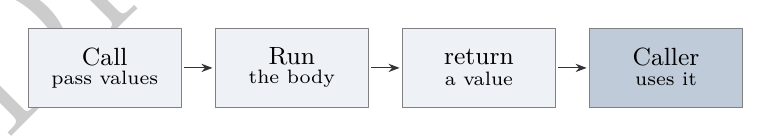
\begin{tikzpicture}[line join=round]
\filldraw[draw=black!50,fill=Paperblue] (0.072,-0.180) rectangle (2.016,-1.188);
\node[,inner sep=1pt,font=\small] at (1.044,-0.540) {Call};
\node[,inner sep=1pt,font=\scriptsize] at (1.044,-0.828) {pass values};
\draw[-{Stealth[length=4pt]},black!80] (2.052,-0.684) -- (2.412,-0.684);
\filldraw[draw=black!50,fill=Paperblue] (2.448,-0.180) rectangle (4.392,-1.188);
\node[,inner sep=1pt,font=\small] at (3.420,-0.540) {Run};
\node[,inner sep=1pt,font=\scriptsize] at (3.420,-0.828) {the body};
\draw[-{Stealth[length=4pt]},black!80] (4.428,-0.684) -- (4.788,-0.684);
\filldraw[draw=black!50,fill=Paperblue] (4.824,-0.180) rectangle (6.768,-1.188);
\node[,inner sep=1pt,font=\small] at (5.796,-0.540) {return};
\node[,inner sep=1pt,font=\scriptsize] at (5.796,-0.828) {a value};
\draw[-{Stealth[length=4pt]},black!80] (6.804,-0.684) -- (7.164,-0.684);
\filldraw[draw=black!50,fill=FAUblue!25] (7.200,-0.180) rectangle (9.144,-1.188);
\node[,inner sep=1pt,font=\small] at (8.172,-0.540) {Caller};
\node[,inner sep=1pt,font=\scriptsize] at (8.172,-0.828) {uses it};
\end{tikzpicture}\par\smallskip{\small\raggedright \textbf{A call.} The caller waits while the body runs, then continues with the returned value; with no \texttt{return} that value is \texttt{None}.\par}\end{minipage}
\end{center}

\Needspace{10\baselineskip}
\begin{center}\small\begin{tabularx}{\linewidth}{>{\raggedright\arraybackslash}X>{\raggedright\arraybackslash}X}\toprule
\textbf{\texttt{return}} & \textbf{\texttt{print}} \\ \midrule
Has meaning only inside a function & Can be used anywhere \\
Only one runs per call & Can run many times in one call \\
Code after it in the block never runs & Code after it runs as normal \\
Its value goes to the caller & Its value goes to the console \\
\bottomrule\end{tabularx}\end{center}

\Needspace{10\baselineskip}
The lecture’s second \texttt{is\_even} has the body \texttt{i\%2 == 0} and no \texttt{return}. The comparison is worked out and thrown away, and the call returns \texttt{None}. So \texttt{print(is\_even(4))} prints \texttt{None}, not \texttt{True}.

\begin{workedbox}{Worked example \ensuremath{\cdot} print inside, print outside}
\Needspace{7\baselineskip}
\begin{enumerate}
\item \texttt{def sq(x): print(x * x)}, then \texttt{y = sq(3)}: the body prints \texttt{9}.
\item The body ends without a \texttt{return}, so \texttt{sq(3)} is \texttt{None} and \texttt{y} is bound to \texttt{None}.
\item \texttt{print(y)} prints \texttt{None}. The output is \texttt{9}, then \texttt{None}.
\item Check: replace the body by \texttt{return x * x} and the output becomes just \texttt{9}, from \texttt{print(y)}.
\end{enumerate}
\end{workedbox}

\Needspace{6\baselineskip}
\begin{notebox}\textbf{Trap:} \texttt{double(3) + 1} with \texttt{def double(x): print(2 * x)} prints 6 and then fails: \texttt{None + 1} raises a \texttt{TypeError}. Seeing the number on screen does not mean the caller got it.\end{notebox}

\Needspace{5\baselineskip}
\begin{notebox}\textbf{Near miss:} in the shell, a bare call such as \texttt{is\_even(3)} shows \texttt{False}, which looks like printing. It is the shell echoing the returned value; in a script nothing appears.\end{notebox}

\Needspace{9\baselineskip}
\begin{recallbox}{Recall check \ensuremath{\cdot} answer without looking}
\Needspace{4\baselineskip}
\begin{enumerate}
\item What does \texttt{print(is\_even(4))} show when \texttt{is\_even} has no \texttt{return}?
\item A function body is \texttt{return 1} followed by \texttt{print("hi")}. What does a call print?
\end{enumerate}

\nopagebreak[4]{\small\itshape Answers: see “7.3 return versus print” under Answers at the end.}
\end{recallbox}
\end{keepsection}

\begin{keepsection}
\Needspace{12\baselineskip}
\section{7.4 Scope}

\Needspace{9\baselineskip}
Functions use names too; you need to know which names a function sees and which ones it changes.

\Needspace{14\baselineskip}
\begin{plainbox}\textbf{In plain words:} every call gets a fresh \textbf{frame} (also called a \textbf{scope} or \textbf{environment}): a table that maps names to objects. The \textbf{formal parameter}, the name in the \texttt{def} line, is bound in that frame to the value of the \textbf{actual parameter}, the argument in the call. Names assigned inside the function live only in its frame and vanish when the call ends. A function can \textbf{read} a name from the main program, but assigning to a name inside a function always means a local name.\end{plainbox}

\begin{equationcard}{Which name is meant}
\[ \begin{gathered} \text{assigned}\, \text{anywhere}\, \text{in}\, \text{the}\, \text{function}\, \to \, \text{local}\, \text{name}\, \text{in}\, \text{the}\, \text{call}’\mathrm{s}\, \text{frame} \\ \text{only}\, \text{read}\, \text{in}\, \text{the}\, \text{function}\, \to \, \text{looked}\, \text{up}\, \text{in}\, \text{the}\, \text{main}\, \text{program}’\mathrm{s}\, \text{frame} \end{gathered} \]
{\small \emph{Read it as: “a name the function assigns is its own; a name it only reads comes from outside”.}\par  Python decides this for the whole function before it runs, so reading a local name before its assignment raises an \texttt{UnboundLocalError}.}
\end{equationcard}

\Needspace{14\baselineskip}
\begin{center}
\begin{minipage}[t]{0.950\linewidth}\centering
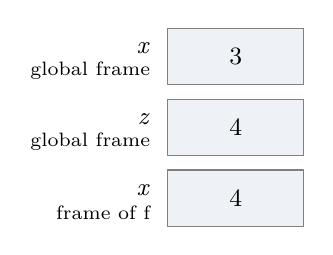
\begin{tikzpicture}[line join=round]
\node[anchor=east,inner sep=1pt,font=\small] at (1.800,-0.432) {\textit{x}};
\node[anchor=east,inner sep=1pt,font=\scriptsize] at (1.800,-0.720) {global frame};
\draw[black!50,fill=Paperblue] (1.980,-0.180) rectangle (3.708,-0.900);
\node[,inner sep=1pt,font=\small] at (2.844,-0.540) {3};
\node[anchor=east,inner sep=1pt,font=\small] at (1.800,-1.332) {\textit{z}};
\node[anchor=east,inner sep=1pt,font=\scriptsize] at (1.800,-1.620) {global frame};
\draw[black!50,fill=Paperblue] (1.980,-1.080) rectangle (3.708,-1.800);
\node[,inner sep=1pt,font=\small] at (2.844,-1.440) {4};
\node[anchor=east,inner sep=1pt,font=\small] at (1.800,-2.232) {\textit{x}};
\node[anchor=east,inner sep=1pt,font=\scriptsize] at (1.800,-2.520) {frame of f};
\draw[black!50,fill=Paperblue] (1.980,-1.980) rectangle (3.708,-2.700);
\node[,inner sep=1pt,font=\small] at (2.844,-2.340) {4};
\end{tikzpicture}\par\smallskip{\small\raggedright \textbf{After the lecture’s \texttt{z = f(x)}.} The parameter \texttt{x} in \texttt{f}’s frame started as 3 and was rebound to 4; the main program’s \texttt{x} is still 3, and \texttt{z} holds the returned 4.\par}\end{minipage}
\end{center}
\begin{tcolorbox}[colback=Paperblue,colframe=Paperblue,boxrule=0pt,arc=0pt,left=7pt,right=7pt,top=5pt,bottom=5pt]\small\sloppy
\noindent\hspace*{0em}\texttt{def f(x):}\par
\noindent\hspace*{1em}\texttt{x = x + 1}\par
\noindent\hspace*{1em}\texttt{print('in f(x): x =', x)}\par
\noindent\hspace*{1em}\texttt{return x}\par
\noindent\hspace*{0em}\texttt{}\par
\noindent\hspace*{0em}\texttt{x = 3}\par
\noindent\hspace*{0em}\texttt{z = f(x)}\par
\end{tcolorbox}

\Needspace{14\baselineskip}
The lecture’s three scope examples each start with \texttt{x = 5} and call a function with \texttt{x} as the argument. In \texttt{f}, the body assigns \texttt{x = 1} and \texttt{x += 1}: that \texttt{x} is local, so \texttt{f} prints 2 and the main program’s \texttt{x} stays 5. In \texttt{g}, the body only reads \texttt{x}, so it picks up the main program’s 5. In \texttt{h}, the body is \texttt{x += 1}, which assigns, so \texttt{x} is local, but it is read before it has a value: \texttt{UnboundLocalError}.

\begin{workedbox}{Worked example \ensuremath{\cdot} trace the lecture’s z = f(x)}
\Needspace{8\baselineskip}
\begin{enumerate}
\item The main program binds \texttt{x} to 3, then calls \texttt{f(x)}: a new frame opens, and the formal parameter \texttt{x} is bound to 3.
\item In \texttt{f}’s frame, \texttt{x = x + 1} rebinds the local \texttt{x} to 4; the line prints \texttt{in f(x): x = 4}.
\item \texttt{return x} hands back 4, the frame disappears, and the main program binds \texttt{z} to 4.
\item Check: the main program’s \texttt{x} was never touched, so \texttt{print(x, z)} would show \texttt{3 4}.
\end{enumerate}
\end{workedbox}

\Needspace{7\baselineskip}
\begin{notebox}\textbf{Trap:} \texttt{x += 1} inside a function, with \texttt{x} defined only outside, does not change the outer \texttt{x}; it raises an \texttt{UnboundLocalError}, because the assignment makes \texttt{x} local for the whole function.\end{notebox}

\Needspace{6\baselineskip}
\begin{notebox}\textbf{Near miss:} naming the parameter \texttt{x}, like the outer variable, looks as if the function works on the outer \texttt{x}. It gets a copy of the outer \emph{name binding}: rebinding the parameter never rebinds the caller’s name. (A list passed in is another story: §7.9.)\end{notebox}

\Needspace{11\baselineskip}
\begin{recallbox}{Recall check \ensuremath{\cdot} answer without looking}
\Needspace{5\baselineskip}
\begin{enumerate}
\item In the lecture’s \texttt{g}, where does the \texttt{x} in \texttt{print(x)} come from?
\item Why does \texttt{h} fail, although \texttt{x = 5} was set before the call?
\item What is the difference between a formal and an actual parameter?
\end{enumerate}

\nopagebreak[4]{\small\itshape Answers: see “7.4 Scope” under Answers at the end.}
\end{recallbox}
\end{keepsection}

\begin{keepsection}
\Needspace{10\baselineskip}
\section{7.5 Functions as arguments}

\Needspace{7\baselineskip}
A function is an object like a number or a string, so it can be passed to another function and called there.

\Needspace{11\baselineskip}
\begin{plainbox}\textbf{In plain words:} the name of a function, written without brackets, refers to the function object. Passing it as an argument hands over the function itself, not its result. The receiving function can then call it with brackets whenever it likes.\end{plainbox}

\begin{equationcard}{Passing a function}
\[ \begin{gathered} \texttt{func\_c(func\_a)}:\, \text{the}\, \text{parameter}\, \texttt{z}\, \text{is}\, \text{bound}\, \text{to}\, \text{the}\, \text{function}\, \texttt{func\_a} \\ \texttt{z()}\, \text{inside}\, \texttt{func\_c}:\, \text{calls}\, \texttt{func\_a} \end{gathered} \]
{\small \emph{Read it as: “give func\_c the function func\_a; func\_c calls it as z()”.}\par  \texttt{func\_c(func\_a())} would instead call \texttt{func\_a} first and pass its result.}
\end{equationcard}
\begin{tcolorbox}[colback=Paperblue,colframe=Paperblue,boxrule=0pt,arc=0pt,left=7pt,right=7pt,top=5pt,bottom=5pt]\small\sloppy
\noindent\hspace*{0em}\texttt{def func\_a():}\par
\noindent\hspace*{1em}\texttt{print('inside func\_a')}\par
\noindent\hspace*{0em}\texttt{}\par
\noindent\hspace*{0em}\texttt{def func\_b(y):}\par
\noindent\hspace*{1em}\texttt{print('inside func\_b')}\par
\noindent\hspace*{1em}\texttt{return y}\par
\noindent\hspace*{0em}\texttt{}\par
\noindent\hspace*{0em}\texttt{def func\_c(z):}\par
\noindent\hspace*{1em}\texttt{print('inside func\_c')}\par
\noindent\hspace*{1em}\texttt{return z()}\par
\noindent\hspace*{0em}\texttt{}\par
\noindent\hspace*{0em}\texttt{print(func\_a())}\par
\noindent\hspace*{0em}\texttt{print(5 + func\_b(2))}\par
\noindent\hspace*{0em}\texttt{print(func\_c(func\_a))}\par
\end{tcolorbox}

\Needspace{12\baselineskip}
\texttt{func\_a} takes no parameters, \texttt{func\_b} takes one, and \texttt{func\_c} takes one that is itself a function. The three \texttt{print} lines show the output of each call followed by its value.

\begin{workedbox}{Worked example \ensuremath{\cdot} the lecture’s three prints}
\Needspace{9\baselineskip}
\begin{enumerate}
\item \texttt{print(func\_a())}: the call prints \texttt{inside func\_a} and returns \texttt{None}, so the next line is \texttt{None}.
\item \texttt{print(5 + func\_b(2))}: the call prints \texttt{inside func\_b} and returns 2; then 5 + 2 is printed: \texttt{7}.
\item \texttt{print(func\_c(func\_a))}: \texttt{func\_c} prints \texttt{inside func\_c}, then \texttt{z()} calls \texttt{func\_a}, which prints \texttt{inside func\_a} and returns \texttt{None}; \texttt{func\_c} returns that \texttt{None}, which is printed.
\item Check: seven lines in all, 2 + 2 + 3, in the order the calls start: inside func\_a, None, inside func\_b, 7, inside func\_c, inside func\_a, None.
\end{enumerate}
\end{workedbox}

\Needspace{6\baselineskip}
\begin{notebox}\textbf{Trap:} \texttt{func\_c(func\_a())} calls \texttt{func\_a} first and passes \texttt{None}; then \texttt{z()} tries to call \texttt{None} and raises a \texttt{TypeError}.\end{notebox}

\Needspace{11\baselineskip}
\begin{notebox}\textbf{Near miss:} \texttt{print(func\_a)} looks like it calls \texttt{func\_a}, but without brackets it prints the function object itself, something like \texttt{\ensuremath{<}function func\_a at 0x…\ensuremath{>}}.\end{notebox}

\begin{recallbox}{Recall check \ensuremath{\cdot} answer without looking}
\Needspace{4\baselineskip}
\begin{enumerate}
\item What is the difference between \texttt{func\_c(func\_a)} and \texttt{func\_c(func\_a())}?
\item With \texttt{def twice(f, x): return f(f(x))} and \texttt{def inc(n): return n + 1}, what is \texttt{twice(inc, 0)}?
\end{enumerate}

\nopagebreak[4]{\small\itshape Answers: see “7.5 Functions as arguments” under Answers at the end.}
\end{recallbox}
\end{keepsection}

\begin{keepsection}
\Needspace{10\baselineskip}
\section{7.6 Tuples}

\Needspace{7\baselineskip}
A function returns one value; a tuple bundles several values into one, so it can return them all.

\Needspace{11\baselineskip}
\begin{plainbox}\textbf{In plain words:} a \textbf{tuple} is an ordered sequence of elements, which may have different types, written in round brackets: \texttt{(2, "fau", 3)}. It is \textbf{immutable}, like a string: you cannot change an element, only build a new tuple. Indexing, slicing, \texttt{len} and \texttt{+} work exactly as for strings.\end{plainbox}

\begin{equationcard}{Tuple operations}
\[ \begin{gathered} \texttt{t = (2, "fau", 3)}:\, \texttt{t[0]}\, \to \, \texttt{2},\, \texttt{len(t)}\, \to \, \texttt{3} \\ \texttt{t[1:2]}\, \to \, \texttt{("fau",)},\, \texttt{t[1:3]}\, \to \, \texttt{("fau", 3)} \\ \texttt{(2, "fau", 3) + (5, 6)}\, \to \, \texttt{(2, "fau", 3, 5, 6)} \end{gathered} \]
{\small \emph{Read it as: “index, slice, length and concatenation as for strings”.}\par  A slice of a tuple is a tuple. \texttt{()} is the empty tuple, and \texttt{("fau",)} with its extra comma is a tuple with one element.}
\end{equationcard}

\begin{equationcard}{Packing and unpacking}
\[ \begin{gathered} \texttt{(x, y) = (y, x)}:\, \text{swap}\, \text{two}\, \text{names} \\ \texttt{return (q, r)},\, \text{then}\, \texttt{(quot, rem) = f(…)} \end{gathered} \]
{\small \emph{Read it as: “build a tuple on the right, then bind each name on the left to one element”.}\par  The right side is worked out completely before any name is bound, which is why the swap works.}
\end{equationcard}

\Needspace{8\baselineskip}
\texttt{t[1] = 4} raises a \texttt{TypeError}: a tuple does not support item assignment. To “change” one, build a new tuple, for example \texttt{t = t[:1] + (4,) + t[2:]}.

\Needspace{12\baselineskip}
The lecture’s \texttt{get\_data} iterates over a tuple of (int, string) pairs. It starts with two empty tuples and grows them with \texttt{nums = nums + (t[0],)}, adding a one-element tuple each round, and adds a word only if it is \texttt{not in words} yet. It returns \texttt{(min\_n, max\_n, unique\_words)}: the smallest and largest number and the count of distinct words.

\begin{workedbox}{Worked example \ensuremath{\cdot} return two values}
\Needspace{7\baselineskip}
\begin{enumerate}
\item \texttt{quotient\_and\_remainder(4, 5)} computes \texttt{q = 4 // 5}, which is 0, and \texttt{r = 4 \% 5}, which is 4.
\item \texttt{return (q, r)} hands back the single tuple \texttt{(0, 4)}.
\item \texttt{(quot, rem) = (0, 4)} unpacks it: \texttt{quot} is 0, \texttt{rem} is 4.
\item Check: 5 \ensuremath{\cdot} 0 + 4 = 4, so quotient and remainder rebuild the dividend.
\end{enumerate}
\end{workedbox}

\Needspace{6\baselineskip}
\begin{notebox}\textbf{Trap:} the swap \texttt{x = y} then \texttt{y = x} loses a value: after the first line both names hold \texttt{y}’s value. Use a temporary name, or \texttt{(x, y) = (y, x)}.\end{notebox}

\Needspace{5\baselineskip}
\begin{notebox}\textbf{Near miss:} \texttt{(5)} looks like a one-element tuple, but brackets alone only group: it is the int 5. The comma makes the tuple: \texttt{(5,)}.\end{notebox}

\Needspace{10\baselineskip}
\begin{recallbox}{Recall check \ensuremath{\cdot} answer without looking}
\Needspace{4\baselineskip}
\begin{enumerate}
\item What are \texttt{t[1:2]} and \texttt{t[1:3]} for \texttt{t = (2, "fau", 3)}?
\item Why does \texttt{(x, y) = (y, x)} swap correctly when \texttt{x = y; y = x} does not?
\end{enumerate}

\nopagebreak[4]{\small\itshape Answers: see “7.6 Tuples” under Answers at the end.}
\end{recallbox}
\end{keepsection}

\begin{keepsection}
\Needspace{10\baselineskip}
\section{7.7 Lists}

\Needspace{7\baselineskip}
Many tasks need a sequence that grows, shrinks and changes; the list is that sequence.

\Needspace{12\baselineskip}
\begin{plainbox}\textbf{In plain words:} a \textbf{list} is an ordered sequence written in square brackets, \texttt{[2, 1, 3]}, reached by index like a string or a tuple. Its elements are usually all of one type but may be mixed, and one element may itself be a list. Unlike a tuple, a list is \textbf{mutable}: \texttt{L[1] = 5} changes the list in place, and it stays the same object.\end{plainbox}

\begin{equationcard}{Indexing a list}
\[ \begin{gathered} \texttt{L = [2, 'a', 4, [1, 2]]}:\, \texttt{len(L)}\, \to \, \texttt{4} \\ \texttt{L[0]}\, \to \, \texttt{2},\, \texttt{L[2] + 1}\, \to \, \texttt{5},\, \texttt{L[3]}\, \to \, \texttt{[1, 2]} \end{gathered} \]
{\small \emph{Read it as: “four elements, indexed 0 to 3; the last one is itself a list”.}\par  \texttt{L[4]} raises an \texttt{IndexError}, and an index may be any expression: with \texttt{i = 2}, \texttt{L[i-1]} is \texttt{'a'}.}
\end{equationcard}

\begin{equationcard}{Changing an element}
\[ \begin{gathered} \texttt{L = [2, 1, 3]},\, \text{then}\, \texttt{L[1] = 5}:\, \texttt{L}\, \text{is}\, \texttt{[2, 5, 3]} \end{gathered} \]
{\small \emph{Read it as: “bind position 1 of the list to 5”.}\par  No new list is made; every name pointing at this list sees the change (§7.9).}
\end{equationcard}
\begin{tcolorbox}[colback=Paperblue,colframe=Paperblue,boxrule=0pt,arc=0pt,left=7pt,right=7pt,top=5pt,bottom=5pt]\small\sloppy
\noindent\hspace*{0em}\texttt{total = 0}\par
\noindent\hspace*{0em}\texttt{for i in range(len(L)):}\par
\noindent\hspace*{1em}\texttt{total += L[i]}\par
\noindent\hspace*{0em}\texttt{print(total)}\par
\noindent\hspace*{0em}\texttt{}\par
\noindent\hspace*{0em}\texttt{total = 0}\par
\noindent\hspace*{0em}\texttt{for i in L:}\par
\noindent\hspace*{1em}\texttt{total += i}\par
\noindent\hspace*{0em}\texttt{print(total)}\par
\end{tcolorbox}

\Needspace{12\baselineskip}
Both loops sum the elements. The first walks the indices 0 to \texttt{len(L) - 1}, because \texttt{range(n)} goes from 0 to \textit{n} \ensuremath{-} 1; the second walks the elements directly, as \texttt{for char in s} does for a string. (The slide writes \texttt{print total}, which is Python 2; see the slips list.)

\begin{workedbox}{Worked example \ensuremath{\cdot} reach into a nested list}
\Needspace{7\baselineskip}
\begin{enumerate}
\item With \texttt{L = [2, 'a', 4, [1, 2]]}, \texttt{L[3]} is the inner list \texttt{[1, 2]}.
\item Index that list again: \texttt{L[3][0]} is 1 and \texttt{L[3][1]} is 2.
\item \texttt{len(L[3])} is 2, while \texttt{len(L)} is 4: the inner list counts as one element of the outer one.
\item Check: \texttt{L[3][2]} would raise an \texttt{IndexError}, because the inner list has only indices 0 and 1.
\end{enumerate}
\end{workedbox}

\Needspace{6\baselineskip}
\begin{notebox}\textbf{Trap:} in \texttt{for i in L}, the name \texttt{i} holds elements, not indices; writing \texttt{L[i]} inside that loop looks up the element’s value as a position.\end{notebox}

\Needspace{10\baselineskip}
\begin{notebox}\textbf{Near miss:} \texttt{L[1] = 5} on a list works, so \texttt{s[1] = "x"} on a string or \texttt{t[1] = 5} on a tuple looks fine too; both raise a \texttt{TypeError}, because strings and tuples are immutable.\end{notebox}

\begin{recallbox}{Recall check \ensuremath{\cdot} answer without looking}
\Needspace{4\baselineskip}
\begin{enumerate}
\item What is \texttt{len([1, [2, 3], 4])}?
\item Name one thing a list can do that a tuple cannot.
\end{enumerate}

\nopagebreak[4]{\small\itshape Answers: see “7.7 Lists” under Answers at the end.}
\end{recallbox}
\end{keepsection}

\begin{keepsection}
\Needspace{11\baselineskip}
\section{7.8 List operations}

\Needspace{8\baselineskip}
Lists come with methods to add, remove, convert and sort; the key question for each is whether it changes the list or makes a new one.

\Needspace{12\baselineskip}
\begin{plainbox}\textbf{In plain words:} a \textbf{method} is a function that belongs to an object and is called with a dot: \texttt{L.append(5)}. Everything in Python is an object with data and methods. Most list methods \textbf{mutate} the list, changing it in place, and return \texttt{None}. The operator \texttt{+}, slicing and \texttt{sorted} leave the list alone and return a new one.\end{plainbox}

\begin{equationcard}{Add}
\[ \begin{gathered} \texttt{L.append(x)}:\, \text{add}\, \texttt{x}\, \text{at}\, \text{the}\, \text{end}\, (\text{mutates}) \\ \texttt{L.extend(M)}:\, \text{add}\, \text{every}\, \text{element}\, \text{of}\, \texttt{M}\, \text{at}\, \text{the}\, \text{end}\, (\text{mutates}) \\ \texttt{L1 + L2}:\, \mathrm{a}\, \text{new}\, \text{list};\, \texttt{L1}\, \text{and}\, \texttt{L2}\, \text{unchanged} \end{gathered} \]
{\small \emph{Read it as: “append one item; extend by a whole list; plus builds a new list”.}\par  \texttt{L.append([0, 6])} adds one element, the list \texttt{[0, 6]}; \texttt{L.extend([0, 6])} adds two.}
\end{equationcard}

\begin{equationcard}{Remove}
\[ \begin{gathered} \texttt{del(L[i])}:\, \text{delete}\, \text{the}\, \text{element}\, \text{at}\, \text{index}\, {i} \\ \texttt{L.pop()}:\, \text{remove}\, \text{the}\, \text{last}\, \text{element}\, \text{and}\, \text{return}\, \text{it} \\ \texttt{L.remove(x)}:\, \text{remove}\, \text{the}\, \text{first}\, \text{occurrence}\, \text{of}\, \texttt{x} \end{gathered} \]
{\small \emph{Read it as: “delete by position, pop from the end, remove by value”.}\par  All three mutate. \texttt{remove} raises a \texttt{ValueError} when \texttt{x} is not in the list.}
\end{equationcard}

\begin{equationcard}{Convert and sort}
\[ \begin{gathered} \texttt{list(s)}:\, \text{every}\, \text{character}\, \text{of}\, \texttt{s}\, \text{as}\, \text{an}\, \text{element} \\ \texttt{s.split(c)}:\, \text{split}\, \texttt{s}\, \text{at}\, \text{each}\, \texttt{c};\, \texttt{c.join(L)}:\, \text{glue}\, \text{the}\, \text{strings}\, \text{of}\, \texttt{L}\, \text{with}\, \texttt{c} \\ \texttt{L.sort()},\, \texttt{L.reverse()}:\, \text{mutate},\, \text{return}\, \texttt{None}\, \cdot \, \texttt{sorted(L)}:\, \mathrm{a}\, \text{new}\, \text{sorted}\, \text{list} \end{gathered} \]
{\small \emph{Read it as: “list of characters; split at c, join with c; sort in place or sorted copy”.}\par  \texttt{s.split()} with no argument splits on spaces.}
\end{equationcard}

\Needspace{9\baselineskip}
The lecture runs four removals in order on a list it does not show; its results fit \texttt{L = [2, 1, 3, 6, 3, 7, 0]}. \texttt{L.remove(2)} leaves \texttt{[1, 3, 6, 3, 7, 0]}; \texttt{L.remove(3)} takes only the first 3, leaving \texttt{[1, 6, 3, 7, 0]}; \texttt{del(L[1])} deletes the 6, leaving \texttt{[1, 3, 7, 0]}; \texttt{L.pop()} returns 0 and leaves \texttt{[1, 3, 7]}.

\Needspace{12\baselineskip}
With \texttt{s = "I\ensuremath{<}3 cs"}, \texttt{list(s)} is \texttt{['I', '\ensuremath{<}', '3', ' ', 'c', 's']} (the space is an element too) and \texttt{s.split('\ensuremath{<}')} is \texttt{['I', '3 cs']}. With \texttt{L = ['a', 'b', 'c']}, \texttt{''.join(L)} is \texttt{"abc"} and \texttt{'\_'.join(L)} is \texttt{"a\_b\_c"}.

\begin{workedbox}{Worked example \ensuremath{\cdot} sort versus sorted}
\Needspace{8\baselineskip}
\begin{enumerate}
\item \texttt{L = [9, 6, 0, 3]}; \texttt{sorted(L)} returns the new list \texttt{[0, 3, 6, 9]} and \texttt{L} is still \texttt{[9, 6, 0, 3]}.
\item \texttt{L.sort()} changes \texttt{L} itself to \texttt{[0, 3, 6, 9]} and returns \texttt{None}.
\item \texttt{L.reverse()} then changes \texttt{L} to \texttt{[9, 6, 3, 0]}.
\item Check: \texttt{M = L.sort()} would bind \texttt{M} to \texttt{None}, exactly the lecture’s \texttt{sortedwarm}; assign the result of \texttt{sorted}, never of \texttt{sort}.
\end{enumerate}
\end{workedbox}

\Needspace{5\baselineskip}
\begin{notebox}\textbf{Trap:} \texttt{L = L.sort()} throws the list away: \texttt{L} is now \texttt{None}. Call \texttt{L.sort()} on its own line.\end{notebox}

\Needspace{5\baselineskip}
\begin{notebox}\textbf{Near miss:} \texttt{L.remove(3)} sounds like “remove the element at index 3”, but it removes the value 3. Deleting by index is \texttt{del(L[3])} or \texttt{L.pop(3)}.\end{notebox}

\Needspace{11\baselineskip}
\begin{recallbox}{Recall check \ensuremath{\cdot} answer without looking}
\Needspace{5\baselineskip}
\begin{enumerate}
\item After \texttt{L1 = [2, 1, 3]}, \texttt{L3 = L1 + [4]} and \texttt{L1.extend([0, 6])}, what are \texttt{L1} and \texttt{L3}?
\item What does \texttt{"a b c".split()} give?
\item Which of \texttt{append}, \texttt{+}, \texttt{pop}, \texttt{sorted} and \texttt{reverse} mutate the list?
\end{enumerate}

\nopagebreak[4]{\small\itshape Answers: see “7.8 List operations” under Answers at the end.}
\end{recallbox}
\end{keepsection}

\begin{keepsection}
\Needspace{11\baselineskip}
\section{7.9 Aliasing and cloning}

\Needspace{8\baselineskip}
Because lists can change, it matters whether two names point at one list or at two; this is where list bugs come from.

\Needspace{11\baselineskip}
\begin{plainbox}\textbf{In plain words:} a list is an object in memory, and a variable name only \textbf{points} at it. \texttt{hot = warm} does not copy the list; it makes a second name for the same list, an \textbf{alias}. Any change made through one name, such as \texttt{hot.append('pink')}, is a \textbf{side effect} visible through the other. To get an independent list, \textbf{clone} it: \texttt{chill = cool[:]} builds a new list with the same elements.\end{plainbox}

\begin{equationcard}{Alias or clone}
\[ \begin{gathered} \texttt{b = a}:\, \text{one}\, \text{list},\, \text{two}\, \text{names} \\ \texttt{b = a[:]}:\, \mathrm{a}\, \text{new}\, \text{list}\, \text{holding}\, \text{the}\, \text{same}\, \text{elements} \end{gathered} \]
{\small \emph{Read it as: “b is another name for a; b is a copy of a”.}\par  After an alias, \texttt{b.append(…)} changes \texttt{a} too; after a clone it does not.}
\end{equationcard}

\Needspace{14\baselineskip}
\begin{center}
\begin{minipage}[t]{0.465\linewidth}\centering
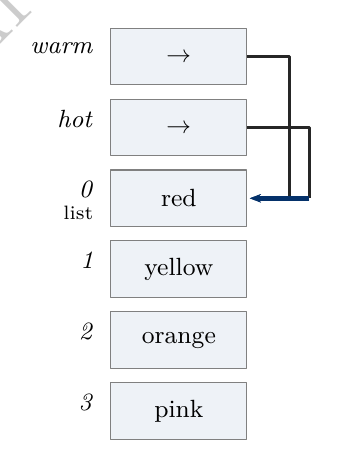
\begin{tikzpicture}[line join=round]
\node[anchor=east,inner sep=1pt,font=\small] at (1.800,-0.432) {\textit{warm}};
\draw[black!50,fill=Paperblue] (1.980,-0.180) rectangle (3.708,-0.900);
\node[,inner sep=1pt,font=\small] at (2.844,-0.540) {\ensuremath{\to}};
\node[anchor=east,inner sep=1pt,font=\small] at (1.800,-1.332) {\textit{hot}};
\draw[black!50,fill=Paperblue] (1.980,-1.080) rectangle (3.708,-1.800);
\node[,inner sep=1pt,font=\small] at (2.844,-1.440) {\ensuremath{\to}};
\node[anchor=east,inner sep=1pt,font=\small] at (1.800,-2.232) {\textit{0}};
\node[anchor=east,inner sep=1pt,font=\scriptsize] at (1.800,-2.520) {list};
\draw[black!50,fill=Paperblue] (1.980,-1.980) rectangle (3.708,-2.700);
\node[,inner sep=1pt,font=\small] at (2.844,-2.340) {red};
\node[anchor=east,inner sep=1pt,font=\small] at (1.800,-3.132) {\textit{1}};
\draw[black!50,fill=Paperblue] (1.980,-2.880) rectangle (3.708,-3.600);
\node[,inner sep=1pt,font=\small] at (2.844,-3.240) {yellow};
\node[anchor=east,inner sep=1pt,font=\small] at (1.800,-4.032) {\textit{2}};
\draw[black!50,fill=Paperblue] (1.980,-3.780) rectangle (3.708,-4.500);
\node[,inner sep=1pt,font=\small] at (2.844,-4.140) {orange};
\node[anchor=east,inner sep=1pt,font=\small] at (1.800,-4.932) {\textit{3}};
\draw[black!50,fill=Paperblue] (1.980,-4.680) rectangle (3.708,-5.400);
\node[,inner sep=1pt,font=\small] at (2.844,-5.040) {pink};
\draw[black!85,line width=1pt] (3.708,-0.540) -- (4.248,-0.540) -- (4.248,-2.340);
\draw[-{Stealth[length=4pt]},FAUblue,line width=1.6pt] (4.248,-2.340) -- (3.744,-2.340);
\draw[black!85,line width=1pt] (3.708,-1.440) -- (4.500,-1.440) -- (4.500,-2.340);
\draw[-{Stealth[length=4pt]},FAUblue,line width=1.6pt] (4.500,-2.340) -- (3.744,-2.340);
\end{tikzpicture}\par\smallskip{\small\raggedright \textbf{The lecture’s alias.} \texttt{warm} and \texttt{hot} point at one list, so \texttt{hot.append('pink')} added the last box for both names.\par}\end{minipage}\hfill
\begin{minipage}[t]{0.465\linewidth}\centering
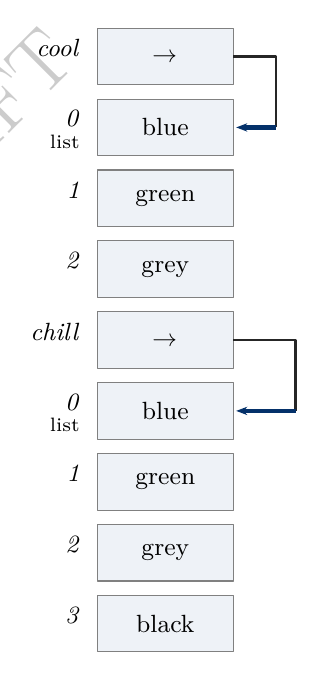
\begin{tikzpicture}[line join=round]
\node[anchor=east,inner sep=1pt,font=\small] at (1.800,-0.432) {\textit{cool}};
\draw[black!50,fill=Paperblue] (1.980,-0.180) rectangle (3.708,-0.900);
\node[,inner sep=1pt,font=\small] at (2.844,-0.540) {\ensuremath{\to}};
\node[anchor=east,inner sep=1pt,font=\small] at (1.800,-1.332) {\textit{0}};
\node[anchor=east,inner sep=1pt,font=\scriptsize] at (1.800,-1.620) {list};
\draw[black!50,fill=Paperblue] (1.980,-1.080) rectangle (3.708,-1.800);
\node[,inner sep=1pt,font=\small] at (2.844,-1.440) {blue};
\node[anchor=east,inner sep=1pt,font=\small] at (1.800,-2.232) {\textit{1}};
\draw[black!50,fill=Paperblue] (1.980,-1.980) rectangle (3.708,-2.700);
\node[,inner sep=1pt,font=\small] at (2.844,-2.340) {green};
\node[anchor=east,inner sep=1pt,font=\small] at (1.800,-3.132) {\textit{2}};
\draw[black!50,fill=Paperblue] (1.980,-2.880) rectangle (3.708,-3.600);
\node[,inner sep=1pt,font=\small] at (2.844,-3.240) {grey};
\node[anchor=east,inner sep=1pt,font=\small] at (1.800,-4.032) {\textit{chill}};
\draw[black!50,fill=Paperblue] (1.980,-3.780) rectangle (3.708,-4.500);
\node[,inner sep=1pt,font=\small] at (2.844,-4.140) {\ensuremath{\to}};
\node[anchor=east,inner sep=1pt,font=\small] at (1.800,-4.932) {\textit{0 }};
\node[anchor=east,inner sep=1pt,font=\scriptsize] at (1.800,-5.220) {list};
\draw[black!50,fill=Paperblue] (1.980,-4.680) rectangle (3.708,-5.400);
\node[,inner sep=1pt,font=\small] at (2.844,-5.040) {blue};
\node[anchor=east,inner sep=1pt,font=\small] at (1.800,-5.832) {\textit{1 }};
\draw[black!50,fill=Paperblue] (1.980,-5.580) rectangle (3.708,-6.300);
\node[,inner sep=1pt,font=\small] at (2.844,-5.940) {green};
\node[anchor=east,inner sep=1pt,font=\small] at (1.800,-6.732) {\textit{2 }};
\draw[black!50,fill=Paperblue] (1.980,-6.480) rectangle (3.708,-7.200);
\node[,inner sep=1pt,font=\small] at (2.844,-6.840) {grey};
\node[anchor=east,inner sep=1pt,font=\small] at (1.800,-7.632) {\textit{3 }};
\draw[black!50,fill=Paperblue] (1.980,-7.380) rectangle (3.708,-8.100);
\node[,inner sep=1pt,font=\small] at (2.844,-7.740) {black};
\draw[black!85,line width=1pt] (3.708,-0.540) -- (4.248,-0.540) -- (4.248,-1.440);
\draw[-{Stealth[length=4pt]},FAUblue,line width=1.6pt] (4.248,-1.440) -- (3.744,-1.440);
\draw[black!85,line width=1pt] (3.708,-4.140) -- (4.500,-4.140) -- (4.500,-5.040);
\draw[-{Stealth[length=4pt]},FAUblue,line width=1.6pt] (4.500,-5.040) -- (3.744,-5.040);
\end{tikzpicture}\par\smallskip{\small\raggedright \textbf{The lecture’s clone.} \texttt{chill = cool[:]} made a second list; \texttt{chill.append('black')} changed only that one.\par}\end{minipage}
\end{center}

\Needspace{10\baselineskip}
Rebinding is different from mutating. \texttt{a = a + [3]} builds a new list and moves the name \texttt{a} to it; an alias \texttt{b} made earlier still points at the old list. \texttt{a.append(3)}, and also \texttt{a += [3]}, change the list itself, so \texttt{b} sees the change.

\Needspace{15\baselineskip}
Lists can hold lists. In the lecture, \texttt{brightcolors = [warm]} and \texttt{brightcolors.append(hot)} put the two lists themselves, not copies, inside \texttt{brightcolors}. After \texttt{hot.append('pink')}, printing \texttt{brightcolors} shows \texttt{[['yellow', 'orange'], ['red', 'pink']]}: side effects reach through nesting too. A list passed to a function is aliased in the same way: the parameter points at the caller’s list.

\begin{workedbox}{Worked example \ensuremath{\cdot} the lecture’s alias and clone}
\Needspace{10\baselineskip}
\begin{enumerate}
\item \texttt{warm = ['red', 'yellow', 'orange']}, then \texttt{hot = warm}: one list, two arrows.
\item \texttt{hot.append('pink')} mutates that list, so \texttt{print(hot)} and \texttt{print(warm)} both show \texttt{['red', 'yellow', 'orange', 'pink']}.
\item \texttt{cool = ['blue', 'green', 'grey']}, then \texttt{chill = cool[:]}: a second list; \texttt{chill.append('black')} changes only it.
\item Check: \texttt{print(chill)} shows four colours, \texttt{print(cool)} still three; \texttt{chill is cool} is \texttt{False} while \texttt{hot is warm} is \texttt{True}.
\end{enumerate}
\end{workedbox}

\Needspace{7\baselineskip}
\begin{notebox}\textbf{Trap:} a function that appends to its list parameter changes the caller’s list. If the caller needs its list unchanged, pass a clone, \texttt{f(L[:])}, or clone inside the function.\end{notebox}

\Needspace{6\baselineskip}
\begin{notebox}\textbf{Near miss:} after \texttt{a = 1}, \texttt{b = a}, \texttt{b = 2}, the lecture shows \texttt{a} is still 1, which looks like the opposite of aliasing. It is not: \texttt{b = 2} rebinds \texttt{b}; it does not change the object. Ints cannot be changed at all, so only rebinding is possible.\end{notebox}

\Needspace{9\baselineskip}
\begin{recallbox}{Recall check \ensuremath{\cdot} answer without looking}
\Needspace{4\baselineskip}
\begin{enumerate}
\item After \texttt{a = [1, 2]}, \texttt{b = a}, \texttt{a = a + [3]}, what is \texttt{b}?
\item Give two ways to clone a list.
\end{enumerate}

\nopagebreak[4]{\small\itshape Answers: see “7.9 Aliasing and cloning” under Answers at the end.}
\end{recallbox}
\end{keepsection}

\begin{keepsection}
\Needspace{10\baselineskip}
\section{7.10 Mutation during iteration}

\Needspace{7\baselineskip}
Changing a list while a \texttt{for} loop walks through it silently skips elements; the fix is to loop over a clone.

\Needspace{10\baselineskip}
\begin{plainbox}\textbf{In plain words:} a \texttt{for} loop over a list keeps a hidden \textbf{counter}: the index of the next element to visit. Removing an element shifts everything after it one place left, but the counter still moves on by one, so the element that slid into the current position is never visited.\end{plainbox}

\begin{equationcard}{Loop over a copy, change the original}
\[ \begin{gathered} \texttt{for e in L1[:]:}\, …\, \texttt{L1.remove(e)} \end{gathered} \]
{\small \emph{Read it as: “walk a snapshot of L1, and remove from the real L1”.}\par  The clone’s length never changes, so every element is visited once.}
\end{equationcard}
\begin{tcolorbox}[colback=Paperblue,colframe=Paperblue,boxrule=0pt,arc=0pt,left=7pt,right=7pt,top=5pt,bottom=5pt]\small\sloppy
\noindent\hspace*{0em}\texttt{def remove\_dups(L1, L2):}\par
\noindent\hspace*{1em}\texttt{for e in L1:}\par
\noindent\hspace*{3em}\texttt{if e in L2:}\par
\noindent\hspace*{5em}\texttt{L1.remove(e)}\par
\noindent\hspace*{0em}\texttt{}\par
\noindent\hspace*{0em}\texttt{L1 = [1, 2, 3, 4]}\par
\noindent\hspace*{0em}\texttt{L2 = [1, 2, 5, 6]}\par
\noindent\hspace*{0em}\texttt{remove\_dups(L1, L2)}\par
\end{tcolorbox}

\Needspace{14\baselineskip}
\begin{center}
\begin{minipage}[t]{0.950\linewidth}\centering
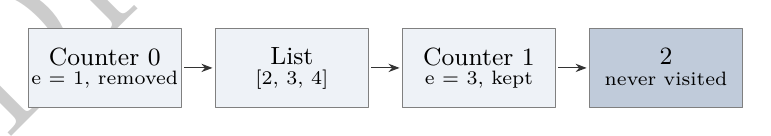
\begin{tikzpicture}[line join=round]
\filldraw[draw=black!50,fill=Paperblue] (0.072,-0.180) rectangle (2.016,-1.188);
\node[,inner sep=1pt,font=\small] at (1.044,-0.540) {Counter 0};
\node[,inner sep=1pt,font=\scriptsize] at (1.044,-0.828) {e = 1, removed};
\draw[-{Stealth[length=4pt]},black!80] (2.052,-0.684) -- (2.412,-0.684);
\filldraw[draw=black!50,fill=Paperblue] (2.448,-0.180) rectangle (4.392,-1.188);
\node[,inner sep=1pt,font=\small] at (3.420,-0.540) {List};
\node[,inner sep=1pt,font=\scriptsize] at (3.420,-0.828) {[2, 3, 4]};
\draw[-{Stealth[length=4pt]},black!80] (4.428,-0.684) -- (4.788,-0.684);
\filldraw[draw=black!50,fill=Paperblue] (4.824,-0.180) rectangle (6.768,-1.188);
\node[,inner sep=1pt,font=\small] at (5.796,-0.540) {Counter 1};
\node[,inner sep=1pt,font=\scriptsize] at (5.796,-0.828) {e = 3, kept};
\draw[-{Stealth[length=4pt]},black!80] (6.804,-0.684) -- (7.164,-0.684);
\filldraw[draw=black!50,fill=FAUblue!25] (7.200,-0.180) rectangle (9.144,-1.188);
\node[,inner sep=1pt,font=\small] at (8.172,-0.540) {2};
\node[,inner sep=1pt,font=\scriptsize] at (8.172,-0.828) {never visited};
\end{tikzpicture}\par\smallskip{\small\raggedright \textbf{The skipped element.} Removing 1 shifts 2 into index 0, but the counter moves on to index 1 and finds 3.\par}\end{minipage}
\end{center}

\Needspace{12\baselineskip}
The intended result is \texttt{[3, 4]}; the buggy loop leaves \texttt{[2, 3, 4]}. The lecture’s fix adds \texttt{L1\_copy = L1[:]} and loops \texttt{for e in L1\_copy:} while still removing from \texttt{L1}. Note that \texttt{L1} inside the function is an alias of the caller’s \texttt{L1} (§7.9), which is why the caller sees the removal at all.

\begin{workedbox}{Worked example \ensuremath{\cdot} trace the hidden counter}
\Needspace{8\baselineskip}
\begin{enumerate}
\item Counter 0: \texttt{e} is 1, which is in \texttt{L2}; \texttt{L1.remove(1)} leaves \texttt{[2, 3, 4]}, and 2 now sits at index 0.
\item Counter 1: \texttt{e} is 3, not in \texttt{L2}. Counter 2: \texttt{e} is 4, not in \texttt{L2}.
\item Counter 3 equals the new length 3, so the loop ends after three rounds; 2 was never visited.
\item Check with the copy: the loop visits 1, 2, 3, 4 from the unchanged clone, removes 1 and 2 from \texttt{L1}, and leaves \texttt{[3, 4]}.
\end{enumerate}
\end{workedbox}

\Needspace{7\baselineskip}
\begin{notebox}\textbf{Trap:} the bug does not always show. Removing even numbers from \texttt{[1, 2, 3, 4]} happens to give the right \texttt{[1, 3]}, but from \texttt{[2, 4, 5]} it gives \texttt{[4, 5]}. Test with neighbouring elements that both match.\end{notebox}

\Needspace{5\baselineskip}
\begin{notebox}\textbf{Near miss:} \texttt{L1\_copy = L1} looks like a copy, but it is an alias (§7.9): the loop still walks the list that shrinks. The copy needs the slice, \texttt{L1[:]}.\end{notebox}

\Needspace{9\baselineskip}
\begin{recallbox}{Recall check \ensuremath{\cdot} answer without looking}
\Needspace{4\baselineskip}
\begin{enumerate}
\item Why does the buggy \texttt{remove\_dups} never see the element 2?
\item Why does \texttt{L1\_copy = L1} not fix the bug?
\end{enumerate}

\nopagebreak[4]{\small\itshape Answers: see “7.10 Mutation during iteration” under Answers at the end.}
\end{recallbox}
\end{keepsection}

\begin{keepsection}
\Needspace{21\baselineskip}
\section{Formula map and units}

\Needspace{10\baselineskip}
\begin{center}\small\begin{tabularx}{\linewidth}{>{\raggedright\arraybackslash}X>{\raggedright\arraybackslash}X}\toprule
\textbf{Rule} & \textbf{Result or meaning} \\ \midrule
\texttt{def f(p):} … \texttt{f(a)} & \texttt{p} bound to \texttt{a} in a new frame; the body runs only at the call \\
value of a call & the \texttt{return} value, else \texttt{None} \\
name assigned in a function & local to each call; only read \ensuremath{\to} taken from the main program \\
\texttt{()}, \texttt{(x,)}, \texttt{(x, y)} & tuples with 0, 1 and 2 elements; immutable \\
\texttt{(a, b) = expr} & unpack; the right side is evaluated first \\
\texttt{append}, \texttt{extend}, \texttt{remove}, \texttt{pop}, \texttt{del}, \texttt{sort}, \texttt{reverse}, \texttt{L[i] = v}, \texttt{L += M} & mutate the list; all but \texttt{pop} return \texttt{None} \\
\texttt{L1 + L2}, \texttt{L[:]}, \texttt{sorted(L)}, \texttt{list(L)} & new lists; the original is unchanged \\
\texttt{b = a} \ensuremath{\cdot} \texttt{b = a[:]} & alias (same object) \ensuremath{\cdot} clone (new object) \\
\texttt{for e in L:} & hidden counter 0, 1, 2, … checked against the current length \\
\bottomrule\end{tabularx}\end{center}

\begin{notebox}\textbf{Check every answer:} for a call, write down both what it prints and what it returns; for a list, ask whether each line mutated the object or rebound a name, and redraw the arrows; for a loop over a list that changes, track the counter and the current length together.\end{notebox}
\end{keepsection}

\begin{keepsection}
\Needspace{17\baselineskip}
\section{Derive it cold}

\Needspace{14\baselineskip}
\begin{enumerate}
\item Trace \texttt{x = 3}, \texttt{z = f(x)} with the lecture’s \texttt{f}, drawing both frames, and state \texttt{x} and \texttt{z} at the end. \hfill{\small\color{FAUblue}§7.4}
\item Predict the output of the lecture’s \texttt{f}, \texttt{g} and \texttt{h} scope examples and explain each from the local-name rule. \hfill{\small\color{FAUblue}§7.4}
\item Write all output lines of the lecture’s three \texttt{print} calls with \texttt{func\_a}, \texttt{func\_b} and \texttt{func\_c}. \hfill{\small\color{FAUblue}§7.3, §7.5}
\item Apply \texttt{remove(2)}, \texttt{remove(3)}, \texttt{del(L[1])} and \texttt{pop()} in order to \texttt{[2, 1, 3, 6, 3, 7, 0]}. \hfill{\small\color{FAUblue}§7.8}
\item Draw names and objects for the lecture’s \texttt{warm}/\texttt{hot}, \texttt{cool}/\texttt{chill} and \texttt{brightcolors} programs. \hfill{\small\color{FAUblue}§7.9}
\item Trace the buggy and the fixed \texttt{remove\_dups} with the loop counter, and explain the difference. \hfill{\small\color{FAUblue}§7.10}
\end{enumerate}
\end{keepsection}

\begin{keepsection}
\Needspace{13\baselineskip}
\section{Explain it}

\Needspace{10\baselineskip}
\begin{enumerate}
\item Why is code split into functions easier to debug than one long sequence of instructions?
\item Why does a function that prints its result instead of returning it cause errors in the caller?
\item Why does \texttt{x += 1} inside a function fail when \texttt{x} exists only outside, while \texttt{print(x)} works?
\item Why can a function return several values, if \texttt{return} hands back only one object?
\item Why does \texttt{hot.append('pink')} change \texttt{warm}, while \texttt{b = 2} after \texttt{b = a} does not change \texttt{a}?
\item When must you loop over a clone of a list instead of the list itself?
\end{enumerate}

\nopagebreak[4]{\small\itshape Answers: see “Explain it” under Answers at the end.}
\end{keepsection}

\clearpage

\begin{keepsection}
\Needspace{11\baselineskip}
\section{Mixed practice}

\Needspace{8\baselineskip}
Try all 24 problems before opening the answers. The order mixes every section on purpose, so you have to choose the method yourself. Predict each output on paper, then check it in a Python shell.

\begin{enumerate}
\item With \texttt{t = (4, "ab", 7)}, evaluate \texttt{t[1:3]} and \texttt{t[2:3]}.
\item \texttt{def sq(x): print(x * x)}. What do \texttt{y = sq(5)} and then \texttt{print(y)} show?
\item \texttt{L = [3, 1, 2]}, then \texttt{L.append(4)} and \texttt{L.extend([5])}. What does \texttt{print(L, len(L))} show?
\item \texttt{a = [1, 2]}, \texttt{b = a}, \texttt{b[0] = 9}. What is \texttt{a}?
\item \texttt{def f(): print(n)}, then \texttt{n = 7} and \texttt{f()}. What is printed, and why is it not an error?
\item Give two benefits of splitting a program into functions.
\item With \texttt{L = [2, 'a', 4, [1, 2]]}, evaluate \texttt{L[3][0]} and \texttt{len(L[3])}.
\item \texttt{L = [1, 2, 3]}, then \texttt{for e in L: L.remove(e)}. What is \texttt{L} afterwards?
\item A file contains only \texttt{def greet(): print("hi")}. What does running the file print?
\item \texttt{def twice(f, x): return f(f(x))} and \texttt{def inc(n): return n + 1}. What is \texttt{twice(inc, 5)}?
\item \texttt{L = [5, 3, 5, 1]}, then \texttt{L.remove(5)}. What does \texttt{print(L.pop(), L)} show?
\item With \texttt{x = 1} and \texttt{y = 2}, what do \texttt{x = y}, \texttt{y = x}, \texttt{print(x, y)} show? Write a correct swap in one line.
\item \texttt{def f(x):} with the body \texttt{return x + 1} and then \texttt{print("done")}. What does \texttt{f(1)} print, and what is its value?
\item \texttt{c = [1, 2]}, \texttt{d = c[:]}, \texttt{d.append(3)}. What does \texttt{print(c, d)} show?
\item \texttt{x = 3} and \texttt{def h(): x = x * 2}. What happens when \texttt{h()} is called?
\item With \texttt{L = [4, 1, 3]} and \texttt{total = 0}, the loop \texttt{for i in range(len(L)): total += L[i] * i} runs. What is \texttt{total}?
\item \texttt{L1 = [2, 4, 5]}, then \texttt{for e in L1:} with the body \texttt{if e \% 2 == 0: L1.remove(e)}. What is \texttt{L1}?
\item Evaluate \texttt{"a-b-c".split("-")} and \texttt{"+".join(["a", "b", "c"])}.
\item Write a function \texttt{cube(n)} with a docstring, and name each of the lecture’s five parts in it.
\item What does \texttt{(q, r) = quotient\_and\_remainder(17, 5)} bind \texttt{q} and \texttt{r} to?
\item \texttt{warm = ["red"]}, \texttt{bright = [warm]}, \texttt{warm.append("pink")}. What does \texttt{print(bright)} show?
\item \texttt{def double(x): print(2 * x)}. What happens on \texttt{double(3) + 1}?
\item The function \texttt{say} returns the string \texttt{"hi"}; the function \texttt{run(g)} calls \texttt{g} and returns the result with \texttt{"!"} added. What are \texttt{run(say)} and \texttt{run(say())}?
\item \texttt{L = [9, 6, 0, 3]}, \texttt{M = sorted(L)}, \texttt{L.reverse()}. What does \texttt{print(L, M)} show?
\end{enumerate}

\nopagebreak[4]{\small\itshape Answers: see “Mixed practice” under Answers at the end.}
\end{keepsection}

\begin{keepsection}
\section{Exam-style problems}

\begin{keepsection}
\Needspace{4\baselineskip}
\subsection{1 \ensuremath{\cdot} A bonus that leaks \ensuremath{\cdot} 20 minutes}
\begin{tcolorbox}[colback=Paperblue,colframe=Paperblue,boxrule=0pt,arc=0pt,left=7pt,right=7pt,top=5pt,bottom=5pt]\small\sloppy
\noindent\hspace*{0em}\texttt{def add\_bonus(scores, bonus):}\par
\noindent\hspace*{1em}\texttt{for i in range(len(scores)):}\par
\noindent\hspace*{3em}\texttt{scores[i] += bonus}\par
\noindent\hspace*{1em}\texttt{return scores}\par
\noindent\hspace*{0em}\texttt{}\par
\noindent\hspace*{0em}\texttt{base = [50, 70, 90]}\par
\noindent\hspace*{0em}\texttt{new = add\_bonus(base, 5)}\par
\noindent\hspace*{0em}\texttt{new.append(100)}\par
\noindent\hspace*{0em}\texttt{print(base, len(base))}\par
\end{tcolorbox}

\Needspace{7\baselineskip}
\begin{enumerate}
\item What does the program print? Trace the list after each line of the main program.
\item Explain with names and objects why \texttt{base} changed although the main program never assigns to it.
\item Change \texttt{add\_bonus} so that \texttt{base} stays \texttt{[50, 70, 90]} and \texttt{new} gets the bonus.
\item Suppose the \texttt{return} line is deleted. What happens on \texttt{new.append(100)}, and why?
\end{enumerate}

\nopagebreak[4]{\small\itshape Answers: see “Exam-style problems” under Answers at the end.}
\end{keepsection}

\begin{keepsection}
\Needspace{4\baselineskip}
\subsection{2 \ensuremath{\cdot} Counting with tuples \ensuremath{\cdot} 20 minutes}
\begin{tcolorbox}[colback=Paperblue,colframe=Paperblue,boxrule=0pt,arc=0pt,left=7pt,right=7pt,top=5pt,bottom=5pt]\small\sloppy
\noindent\hspace*{0em}\texttt{def split\_counts(pairs):}\par
\noindent\hspace*{1em}\texttt{names = []}\par
\noindent\hspace*{1em}\texttt{total = 0}\par
\noindent\hspace*{1em}\texttt{for p in pairs:}\par
\noindent\hspace*{3em}\texttt{if p[1] == 0:}\par
\noindent\hspace*{5em}\texttt{pairs.remove(p)}\par
\noindent\hspace*{3em}\texttt{else:}\par
\noindent\hspace*{5em}\texttt{names.append(p[0])}\par
\noindent\hspace*{5em}\texttt{total += p[1]}\par
\noindent\hspace*{1em}\texttt{return (names, total)}\par
\noindent\hspace*{0em}\texttt{}\par
\noindent\hspace*{0em}\texttt{data = [("ann", 2), ("bob", 0), ("cy", 0), ("dee", 3)]}\par
\noindent\hspace*{0em}\texttt{(n, t) = split\_counts(data)}\par
\noindent\hspace*{0em}\texttt{print(n, t, len(data))}\par
\end{tcolorbox}

\Needspace{7\baselineskip}
\begin{enumerate}
\item Trace the loop’s hidden counter and the list \texttt{pairs}, round by round. What is printed?
\item The intention was to remove every pair with a count of 0. Which pair survives, and why?
\item Fix the function with one change, and give the new output.
\item Why is \texttt{p[1] = 1} inside the loop an error, while \texttt{pairs.remove(p)} is allowed?
\end{enumerate}

\nopagebreak[4]{\small\itshape Answers: see “Exam-style problems” under Answers at the end.}
\end{keepsection}
\end{keepsection}

\begin{keepsection}
\Needspace{22\baselineskip}
\section{Slips in the notes}

\Needspace{19\baselineskip}
Each item was checked against the rendered slides and against Python 3. Slide numbers refer to “07\_abstraction\_functions\_tupels\_lists.pdf”.

\Needspace{16\baselineskip}
\begin{itemize}
\item \textbf{Slide 12, docstring.} The docstring of the version without \texttt{return} says “Does not return anything”. The function still returns a value, \texttt{None}, as the same slide then says; read it as “returns nothing useful” (§7.3).
\item \textbf{Slide 15, error message.} The \texttt{h} example is labelled “UnboundLocalError: local variable 'x' referenced before assignment”. That is the wording of Python up to 3.10; Python 3.11 and later say “cannot access local variable 'x' where it is not associated with a value”. The error type is the same (§7.4).
\item \textbf{Slide 21, floor division.} \texttt{x // y} is annotated “integer division”. It is floor division: it rounds down, so \texttt{-7 // 2} is \ensuremath{-}4, and with a float operand the result is a float (Chapter 6, §6.2).
\item \textbf{Slide 26, print.} Both loops end with \texttt{print total}, which is Python 2 syntax; Python 3 raises a \texttt{SyntaxError} and needs \texttt{print(total)} (§7.7).
\item \textbf{Slide 29, missing list.} The four removals run “in order” on a list \texttt{L} that is never shown. The stated results fit \texttt{L = [2, 1, 3, 6, 3, 7, 0]}, which this guide uses (§7.8).
\end{itemize}
\end{keepsection}

\begin{keepsection}
\Needspace{10\baselineskip}
\section{Self-check}

\Needspace{7\baselineskip}
These are the chapter’s learning goals. Tick a skill only in a later session, at least one day after studying, when you can show it without notes.

\begin{itemize}
\item $\mdlgwhtsquare$\ Explain decomposition and abstraction, and what a docstring is for. (6)
\item $\mdlgwhtsquare$\ Write a function with parameters and a docstring, and say when its body runs. (9, 19)
\item $\mdlgwhtsquare$\ Tell what a call prints from what it returns, including \texttt{None}. (2, 13, 22)
\item $\mdlgwhtsquare$\ Trace frames and decide which names are local, including \texttt{UnboundLocalError}. (5, 15)
\item $\mdlgwhtsquare$\ Pass a function as an argument and call it inside another function. (10, 23)
\item $\mdlgwhtsquare$\ Index, slice and concatenate tuples, including one-element tuples. (1)
\item $\mdlgwhtsquare$\ Swap names and return several values with tuple unpacking. (12, 20)
\item $\mdlgwhtsquare$\ Index nested lists and change list elements in place. (7, 16)
\item $\mdlgwhtsquare$\ Apply \texttt{append}, \texttt{extend}, \texttt{+}, \texttt{del}, \texttt{pop} and \texttt{remove} and give the resulting list. (3, 11)
\item $\mdlgwhtsquare$\ Convert with \texttt{list}, \texttt{split} and \texttt{join}, and use \texttt{sort} versus \texttt{sorted}. (18, 24)
\item $\mdlgwhtsquare$\ Draw names and objects and predict side effects of aliasing, also in nested lists. (4, 21)
\item $\mdlgwhtsquare$\ Clone a list and tell rebinding from mutation. (14)
\item $\mdlgwhtsquare$\ Trace a loop that mutates its list and fix it with a clone. (8, 17)
\item $\mdlgwhtsquare$\ Rebuild every item in the derivation list on blank paper.
\item $\mdlgwhtsquare$\ Complete both exam-style problems in 20 minutes each.
\end{itemize}
\end{keepsection}


\clearpage
\section{Answers}
\begin{keepsection}\subsection{Start from memory}

\Needspace{10\baselineskip}
\begin{enumerate}
\item \texttt{None}, the value that stands for “no value”. \hfill{\small\color{FAUblue}§7.3}
\item \texttt{(5)} is just the int 5 in brackets; \texttt{(5,)} is a tuple with one element. \hfill{\small\color{FAUblue}§7.6}
\item \texttt{a} becomes \texttt{[1, 2, 3]} too: both names point at the same list. \hfill{\small\color{FAUblue}§7.9}
\item \texttt{L.sort()} sorts \texttt{L} in place and returns \texttt{None}; \texttt{sorted(L)} returns a new sorted list and leaves \texttt{L} alone. \hfill{\small\color{FAUblue}§7.8}
\item It can read it. Assigning to that name inside the function makes a new local name instead, unless the name is declared \texttt{global}. \hfill{\small\color{FAUblue}§7.4}
\end{enumerate}

\end{keepsection}
\begin{keepsection}\subsection{7.1 Decomposition and abstraction}

\Needspace{6\baselineskip}
\begin{enumerate}
\item Decomposition splits a program into self-contained modules; abstraction hides how each module works, so it can be used as a black box.
\item What the inputs must be and what the function returns, so the caller can use it without reading the body.
\end{enumerate}

\end{keepsection}
\begin{keepsection}\subsection{7.2 Defining and calling functions}

\Needspace{4\baselineskip}
\begin{enumerate}
\item A name, parameters (0 or more), a docstring (optional), a body, and a return value.
\item A \texttt{TypeError}: \texttt{is\_even()} is missing 1 required positional argument, \texttt{i}.
\end{enumerate}

\end{keepsection}
\begin{keepsection}\subsection{7.3 return versus print}

\Needspace{4\baselineskip}
\begin{enumerate}
\item \texttt{None}: the comparison is computed but not returned.
\item Nothing: \texttt{return} ends the call, so the \texttt{print} line never runs.
\end{enumerate}

\end{keepsection}
\begin{keepsection}\subsection{7.4 Scope}

\Needspace{6\baselineskip}
\begin{enumerate}
\item From the main program’s frame, because \texttt{g} never assigns \texttt{x}.
\item \texttt{x += 1} assigns \texttt{x}, so \texttt{x} is local in \texttt{h}; the local \texttt{x} has no value when \texttt{+=} reads it.
\item The formal parameter is the name in the \texttt{def} line; the actual parameter is the value given in the call, which the formal one is bound to.
\end{enumerate}

\end{keepsection}
\begin{keepsection}\subsection{7.5 Functions as arguments}

\Needspace{5\baselineskip}
\begin{enumerate}
\item The first passes the function so \texttt{func\_c} can call it; the second calls \texttt{func\_a} first and passes its result, \texttt{None}.
\item 2: \texttt{inc(0)} is 1, and \texttt{inc(1)} is 2.
\end{enumerate}

\end{keepsection}
\begin{keepsection}\subsection{7.6 Tuples}

\Needspace{5\baselineskip}
\begin{enumerate}
\item \texttt{("fau",)} and \texttt{("fau", 3)}, both tuples.
\item The right side \texttt{(y, x)} is built from the old values before either name is rebound; the two-line version overwrites \texttt{x} before \texttt{y} reads it.
\end{enumerate}

\end{keepsection}
\begin{keepsection}\subsection{7.7 Lists}

\Needspace{4\baselineskip}
\begin{enumerate}
\item 3: the inner list is one element.
\item Change in place, for example \texttt{L[0] = 9} or \texttt{L.append(9)}.
\end{enumerate}

\end{keepsection}
\begin{keepsection}\subsection{7.8 List operations}

\Needspace{5\baselineskip}
\begin{enumerate}
\item \texttt{L1} is \texttt{[2, 1, 3, 0, 6]}; \texttt{L3} is \texttt{[2, 1, 3, 4]}, a separate list made before the extend.
\item \texttt{['a', 'b', 'c']}: with no argument, runs of spaces count as one separator.
\item \texttt{append}, \texttt{pop} and \texttt{reverse}; \texttt{+} and \texttt{sorted} make new lists.
\end{enumerate}

\end{keepsection}
\begin{keepsection}\subsection{7.9 Aliasing and cloning}

\Needspace{4\baselineskip}
\begin{enumerate}
\item \texttt{[1, 2]}: \texttt{a + [3]} is a new list, and only \texttt{a} moved to it.
\item \texttt{b = a[:]}, as in the lecture, or \texttt{b = list(a)}.
\end{enumerate}

\end{keepsection}
\begin{keepsection}\subsection{7.10 Mutation during iteration}

\Needspace{4\baselineskip}
\begin{enumerate}
\item Removing 1 shifts 2 to index 0, but the loop’s counter moves on to index 1.
\item It makes an alias, not a clone; the loop still walks the same list that is being shortened.
\end{enumerate}

\end{keepsection}
\begin{keepsection}\subsection{Explain it}

\Needspace{16\baselineskip}
\begin{enumerate}
\item Each function is small, has a stated input and output, and can be tested alone; once it works, every call to it works, so a bug is found in one place. \hfill{\small\color{FAUblue}§7.1}
\item The caller receives \texttt{None}, not the number on screen, so any further use, such as \texttt{result + 1}, fails or computes with \texttt{None}. \hfill{\small\color{FAUblue}§7.3}
\item An assignment anywhere in the function makes the name local for the whole function, so \texttt{x += 1} reads a local \texttt{x} that has no value yet. A name that is only read is looked up in the main program. \hfill{\small\color{FAUblue}§7.4}
\item It returns one tuple that holds them all, and the caller unpacks it into several names. \hfill{\small\color{FAUblue}§7.6}
\item \texttt{append} mutates the one list that both names point at. \texttt{b = 2} only moves the name \texttt{b} to another object; nothing is mutated. \hfill{\small\color{FAUblue}§7.9}
\item When the loop body adds or removes elements of that list: the hidden counter does not adjust to the new positions, so elements are skipped or visited twice. \hfill{\small\color{FAUblue}§7.10}
\end{enumerate}

\end{keepsection}
\begin{keepsection}\subsection{Mixed practice}

\begin{enumerate}
\item \texttt{('ab', 7)} and \texttt{(7,)}: slices of a tuple are tuples, and a one-element tuple prints with its comma. \hfill{\small\color{FAUblue}§7.6}
\item \texttt{25}, then \texttt{None}: the body prints, but without a \texttt{return} the call’s value is \texttt{None}. \hfill{\small\color{FAUblue}§7.3}
\item \texttt{[3, 1, 2, 4, 5] 5}: \texttt{append} adds one element and \texttt{extend} adds each element of \texttt{[5]}. \hfill{\small\color{FAUblue}§7.8}
\item \texttt{[9, 2]}: \texttt{b} is an alias, so changing an element through \texttt{b} changes the one list. \hfill{\small\color{FAUblue}§7.9}
\item \texttt{7}: \texttt{f} only reads \texttt{n}, so it looks it up in the main program, where \texttt{n} is bound by the time \texttt{f} is called. \hfill{\small\color{FAUblue}§7.4}
\item Code is written and debugged once and reused by calling it; the program stays organised, and each piece can be used as a black box through its docstring. \hfill{\small\color{FAUblue}§7.1}
\item 1 and 2: \texttt{L[3]} is the inner list \texttt{[1, 2]}. \hfill{\small\color{FAUblue}§7.7}
\item \texttt{[2]}: counter 0 removes 1 (list \texttt{[2, 3]}), counter 1 finds 3 and removes it (list \texttt{[2]}), counter 2 is past the end. \hfill{\small\color{FAUblue}§7.10}
\item Nothing: the file only defines the function and never calls it. \hfill{\small\color{FAUblue}§7.2}
\item 7: \texttt{inc(5)} is 6, then \texttt{inc(6)} is 7. \hfill{\small\color{FAUblue}§7.5}
\item \texttt{1 [3, 5]}: \texttt{remove(5)} takes the first 5 only, leaving \texttt{[3, 5, 1]}; \texttt{pop()} returns 1 and removes it. \hfill{\small\color{FAUblue}§7.8}
\item \texttt{2 2}: \texttt{x = y} overwrites 1 before it is saved. Correct: \texttt{(x, y) = (y, x)}. \hfill{\small\color{FAUblue}§7.6}
\item Nothing, and its value is 2: \texttt{return} ends the call before the \texttt{print} line. \hfill{\small\color{FAUblue}§7.3}
\item \texttt{[1, 2] [1, 2, 3]}: \texttt{c[:]} is a clone, so \texttt{append} changes only \texttt{d}. \hfill{\small\color{FAUblue}§7.9}
\item An \texttt{UnboundLocalError}: the assignment makes \texttt{x} local in \texttt{h}, and the right side reads it before it has a value. \hfill{\small\color{FAUblue}§7.4}
\item 7: 4 \ensuremath{\cdot} 0 + 1 \ensuremath{\cdot} 1 + 3 \ensuremath{\cdot} 2 = 0 + 1 + 6. \hfill{\small\color{FAUblue}§7.7}
\item \texttt{[4, 5]}: counter 0 removes 2, shifting 4 to index 0; counter 1 finds 5, which stays. The 4 is never checked. \hfill{\small\color{FAUblue}§7.10}
\item \texttt{['a', 'b', 'c']} and \texttt{"a+b+c"}. \hfill{\small\color{FAUblue}§7.8}
\item \texttt{def cube(n):} gives the name \texttt{cube} and one parameter \texttt{n}; next, \texttt{"""Input: n, an int. Returns n cubed."""} is the docstring; \texttt{return n ** 3} is the body and what it returns. \hfill{\small\color{FAUblue}§7.2}
\item \texttt{q} is 3 and \texttt{r} is 2, because 17 = 5 \ensuremath{\cdot} 3 + 2. \hfill{\small\color{FAUblue}§7.6}
\item \texttt{[['red', 'pink']]}: \texttt{bright} holds the list \texttt{warm} itself, not a copy. \hfill{\small\color{FAUblue}§7.9}
\item It prints 6, then raises a \texttt{TypeError}: \texttt{double(3)} is \texttt{None}, and \texttt{None + 1} is not defined. \hfill{\small\color{FAUblue}§7.3}
\item \texttt{"hi!"}; and a \texttt{TypeError}, because \texttt{say()} passes the string \texttt{"hi"}, and \texttt{g()} tries to call a string. \hfill{\small\color{FAUblue}§7.5}
\item \texttt{[3, 0, 6, 9] [0, 3, 6, 9]}: \texttt{sorted} made a separate list before \texttt{reverse} mutated \texttt{L}. \hfill{\small\color{FAUblue}§7.8}
\end{enumerate}

\end{keepsection}
\begin{keepsection}\subsection{Exam-style problems}

\Needspace{12\baselineskip}
\begin{enumerate}
\item The loop adds 5 to each element: \texttt{[55, 75, 95]}. \texttt{new} then gets 100 appended to the same list, so the program prints \texttt{[55, 75, 95, 100] 4}. \hfill{\small\color{FAUblue}§7.7, §7.8}
\item The parameter \texttt{scores} points at the caller’s list, so \texttt{scores[i] += bonus} mutates it. The function returns that same list, so \texttt{new} is a third name for it, and \texttt{new.append(100)} changes it again. Only one list exists. \hfill{\small\color{FAUblue}§7.4, §7.9}
\item Clone first: \texttt{result = scores[:]}, then add the bonus to \texttt{result[i]} in the loop and \texttt{return result}. Now \texttt{new} is a different list, and \texttt{base} is untouched. \hfill{\small\color{FAUblue}§7.9}
\item The call returns \texttt{None}, so \texttt{new} is \texttt{None} and \texttt{new.append(100)} raises an \texttt{AttributeError}: \texttt{None} has no method \texttt{append}. (The bonus was still added to \texttt{base}.) \hfill{\small\color{FAUblue}§7.3}
\end{enumerate}

\end{keepsection}
\begin{keepsection}\subsection{Exam-style problems}

\Needspace{12\baselineskip}
\begin{enumerate}
\item Counter 0: ann, count 2, so \texttt{names} is \texttt{['ann']} and \texttt{total} 2. Counter 1: bob, count 0, removed; the list is now ann, cy, dee. Counter 2: dee, count 3, so \texttt{names} is \texttt{['ann', 'dee']} and \texttt{total} 5. Counter 3 equals the length 3: done. It prints \texttt{['ann', 'dee'] 5 3}. \hfill{\small\color{FAUblue}§7.10, §7.6}
\item \texttt{("cy", 0)} survives. Removing bob shifted cy into index 1, and the counter moved on to index 2, so cy was never tested. \hfill{\small\color{FAUblue}§7.10}
\item Loop over a clone: \texttt{for p in pairs[:]:}. Every pair is visited, both zero pairs are removed from \texttt{data}, and it prints \texttt{['ann', 'dee'] 5 2}. \hfill{\small\color{FAUblue}§7.10, §7.9}
\item \texttt{p} is a tuple, which is immutable, so assigning to \texttt{p[1]} raises a \texttt{TypeError}. \texttt{pairs} is a list, which is mutable, so removing one of its elements is allowed. \hfill{\small\color{FAUblue}§7.6, §7.7}
\end{enumerate}

\end{keepsection}

\vfill{\small Personal study guide based on the supplied “07\_abstraction\_functions\_tupels\_lists.pdf” (39 slides, lecture dated 3 May 2024; the slides credit MIT OpenCourseWare 6.0001), written in my own words; no lecture pages or figures are reproduced. Not an official FAU publication; check course details against the current notes. Made by \textbf{Thanate Amornjiraporn (Focus)}.}

\end{document}
